\section*{Ejercicio 9}

\subsection*{Analizar filtro recursivo de segundo orden sin emplear Transformada Z:}

\begin{figure}[H]
    \centering 
    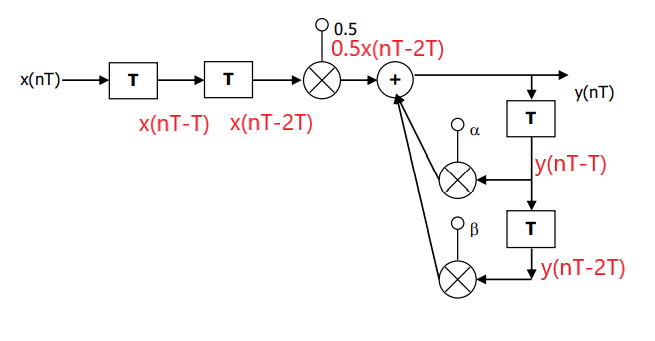
\includegraphics [scale=0.8]{images/ej9.png} 
    \caption{Diagrama}
\end{figure}

La señal de salida del sistema se puede obtener inspeccionando el diagrama, de modo que:

$$y(nT) = \frac{1}{2}x(T(n-2)) + \alpha y(T(n-1)) + \beta y(T(n-2))$$

Se quiere conocer la respuesta del sistema a las señales impulso unitario $x(nT) = \delta (nT)$, y la  señal escalón $x(nT) = u(nT)$, para el intervalo $0\leq n\leq 30$ considerando los siguientes valores de constantes:

$$
\left\{\begin{matrix}
\alpha  = 1, \beta = -\frac{1}{2} 
\\ 
\alpha  = \frac{1}{2}, \beta = -\frac{1}{8} 
\\ 
\alpha  = \frac{5}{4}, \beta = -\frac{25}{32} 
\end{matrix}\right.
$$

Se computó la respuesta del sistema a las señales mediante simulación en Python. Se presentan los resultados en forma tabular y gráfica para cada caso.

\begin{figure}[H]
    \centering 
    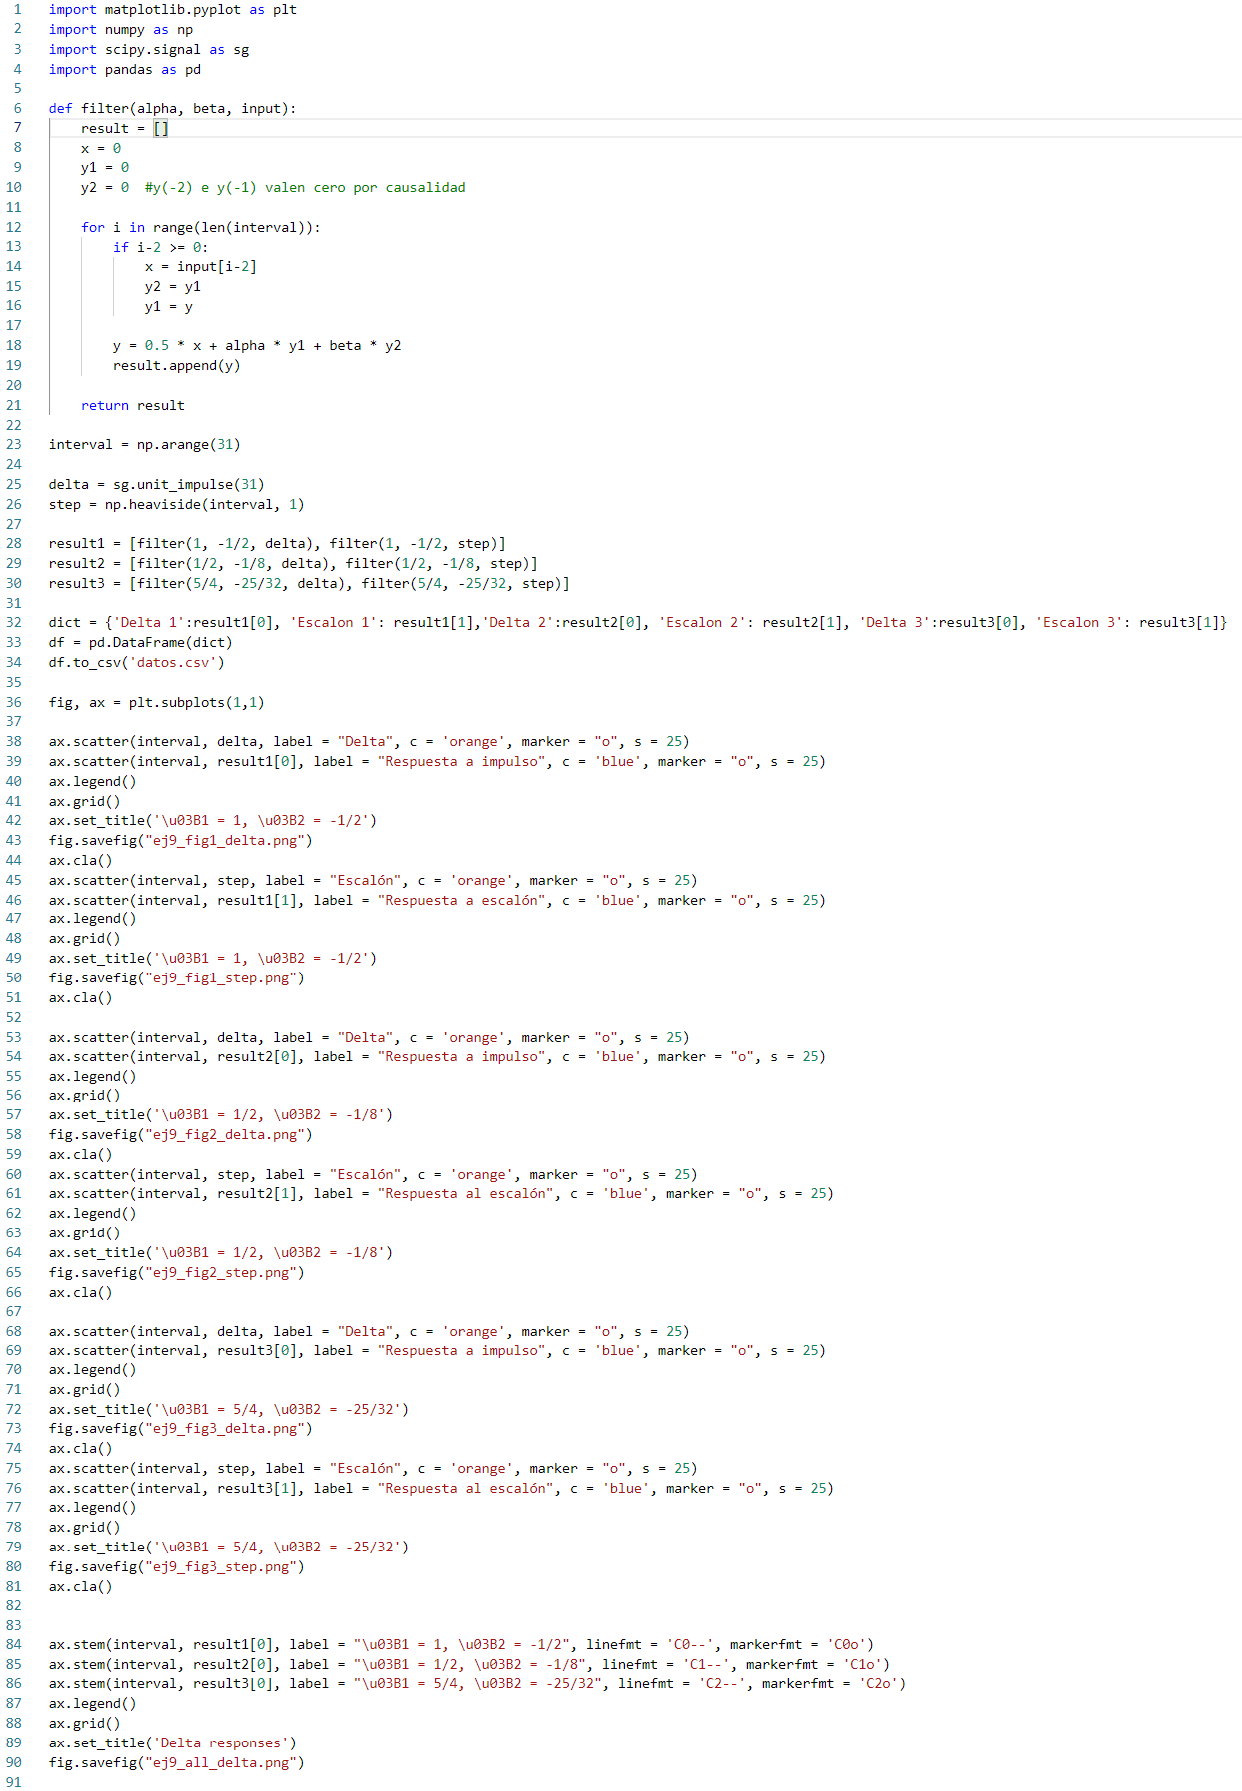
\includegraphics [scale=0.6]{images/9code.png}
    \caption{Código para simulación, tabla y gráficos.} 
\end{figure}

% Please add the following required packages to your document preamble:
% \usepackage[table,xcdraw]{xcolor}
% If you use beamer only pass "xcolor=table" option, i.e. \documentclass[xcolor=table]{beamer}
\begin{table}[H]
    \centering
    \begin{tabular}{c|cccccc|}
    \cline{2-7}
                             & \multicolumn{2}{c|}{\cellcolor[HTML]{C0C0C0}$\alpha  = 1, \beta = -\frac{1}{2}$}  & \multicolumn{2}{c|}{\cellcolor[HTML]{C0C0C0}$\alpha  = \frac{1}{2}, \beta = -\frac{1}{8}$} & \multicolumn{2}{c|}{\cellcolor[HTML]{C0C0C0}$\alpha  = \frac{5}{4}, \beta = -\frac{25}{32}$} \\ \hline
    \multicolumn{1}{|c|}{n}  & \multicolumn{1}{c|}{$x(nT) = \delta (nT)$} & \multicolumn{1}{c|}{$x(nT) = u(nT)$} & \multicolumn{1}{c|}{$x(nT) = \delta (nT)$}      & \multicolumn{1}{c|}{$x(nT) = u(nT)$}     & \multicolumn{1}{c|}{$x(nT) = \delta (nT)$}                 & $x(nT) = u(nT)$                 \\ \hline
    \multicolumn{1}{|c|}{0}  & 0                                          & 0                                    & 0                                               & 0                                        & 0                                                          & 0                               \\ \cline{1-1}
    \multicolumn{1}{|c|}{1}  & 0                                          & 0                                    & 0                                               & 0                                        & 0                                                          & 0                               \\ \cline{1-1}
    \multicolumn{1}{|c|}{2}  & 0.5                                        & 0.5                                  & 0.5                                             & 0.5                                      & 0.5                                                        & 0.5                             \\ \cline{1-1}
    \multicolumn{1}{|c|}{3}  & 0.5                                        & 1                                    & 0.25                                            & 0.75                                     & 0.625                                                      & 1.125                           \\ \cline{1-1}
    \multicolumn{1}{|c|}{4}  & 0.25                                       & 1.25                                 & 0.0625                                          & 0.8125                                   & 0.390625                                                   & 1.515625                        \\ \cline{1-1}
    \multicolumn{1}{|c|}{5}  & 0                                          & 1.25                                 & 0                                               & 0.8125                                   & 0                                                          & 1.515625                        \\ \cline{1-1}
    \multicolumn{1}{|c|}{6}  & -0.125                                     & 1.125                                & -0.0078125                                      & 0.8046875                                & -0.30517578                                                & 1.21044922                      \\ \cline{1-1}
    \multicolumn{1}{|c|}{7}  & -0.125                                     & 1                                    & -0.00390625                                     & 0.80078125                               & -0.38146973                                                & 0.82897949                      \\ \cline{1-1}
    \multicolumn{1}{|c|}{8}  & -0.0625                                    & 0.9375                               & -0.00097656                                     & 0.79980469                               & -0.23841858                                                & 0.59056091                      \\ \cline{1-1}
    \multicolumn{1}{|c|}{9}  & 0                                          & 0.9375                               & 0                                               & 0.79980469                               & 0                                                          & 0.59056091                      \\ \cline{1-1}
    \multicolumn{1}{|c|}{10} & 0.03125                                    & 0.96875                              & 0.00012207                                      & 0.79992676                               & 0.18626451                                                 & 0.77682543                      \\ \cline{1-1}
    \multicolumn{1}{|c|}{11} & 0.03125                                    & 1                                    & 6.10E-05                                        & 0.79998779                               & 0.23283064                                                 & 1.00965607                      \\ \cline{1-1}
    \multicolumn{1}{|c|}{12} & 0.015625                                   & 1.015625                             & 1.53E-05                                        & 0.80000305                               & 0.14551915                                                 & 1.15517522                      \\ \cline{1-1}
    \multicolumn{1}{|c|}{13} & 0                                          & 1.015625                             & 0                                               & 0.80000305                               & 0                                                          & 1.15517522                      \\ \cline{1-1}
    \multicolumn{1}{|c|}{14} & -0.0078125                                 & 1.0078125                            & -1.91E-06                                       & 0.80000114                               & -0.11368684                                                & 1.04148839                      \\ \cline{1-1}
    \multicolumn{1}{|c|}{15} & -0.0078125                                 & 1                                    & -9.54E-07                                       & 0.80000019                               & -0.14210855                                                & 0.89937984                      \\ \cline{1-1}
    \multicolumn{1}{|l|}{16} & -0.00390625                                & 0.99609375                           & -2.38E-07                                       & 0.79999995                               & -0.08881784                                                & 0.810562                        \\ \cline{1-1}
    \multicolumn{1}{|l|}{17} & 0                                          & 0.99609375                           & 0                                               & 0.79999995                               & 0                                                          & 0.810562                        \\ \cline{1-1}
    \multicolumn{1}{|l|}{18} & 0.00195313                                 & 0.99804688                           & 2.98E-08                                        & 0.79999998                               & 0.06938894                                                 & 0.87995094                      \\ \cline{1-1}
    \multicolumn{1}{|l|}{19} & 0.00195313                                 & 1                                    & 1.49E-08                                        & 0.8                                      & 0.08673617                                                 & 0.96668711                      \\ \cline{1-1}
    \multicolumn{1}{|l|}{20} & 0.00097656                                 & 1.00097656                           & 3.73E-09                                        & 0.8                                      & 0.05421011                                                 & 1.02089722                      \\ \cline{1-1}
    \multicolumn{1}{|l|}{21} & 0                                          & 1.00097656                           & 0                                               & 0.8                                      & 0                                                          & 1.02089722                      \\ \cline{1-1}
    \multicolumn{1}{|l|}{22} & -0.00048828                                & 1.00048828                           & -4.66E-10                                       & 0.8                                      & -0.04235165                                                & 0.97854557                      \\ \cline{1-1}
    \multicolumn{1}{|l|}{23} & -0.00048828                                & 1                                    & -2.33E-10                                       & 0.8                                      & -0.05293956                                                & 0.92560601                      \\ \cline{1-1}
    \multicolumn{1}{|l|}{24} & -0.00024414                                & 0.99975586                           & -5.82E-11                                       & 0.8                                      & -0.03308722                                                & 0.89251879                      \\ \cline{1-1}
    \multicolumn{1}{|c|}{25} & 0                                          & 0.99975586                           & 0                                               & 0.8                                      & 0                                                          & 0.89251879                      \\ \cline{1-1}
    \multicolumn{1}{|c|}{26} & 0.00012207                                 & 0.99987793                           & 7.28E-12                                        & 0.8                                      & 0.02584939                                                 & 0.91836818                      \\ \cline{1-1}
    \multicolumn{1}{|c|}{27} & 0.00012207                                 & 1                                    & 3.64E-12                                        & 0.8                                      & 0.03231174                                                 & 0.95067992                      \\ \cline{1-1}
    \multicolumn{1}{|c|}{28} & 6.10E-05                                   & 1.00006104                           & 9.09E-13                                        & 0.8                                      & 0.02019484                                                 & 0.97087476                      \\ \cline{1-1}
    \multicolumn{1}{|c|}{29} & 0                                          & 1.00006104                           & 0                                               & 0.8                                      & -3.47E-18                                                  & 0.97087476                      \\ \cline{1-1}
    \multicolumn{1}{|c|}{30} & -3.05E-05                                  & 1.00003052                           & -1.14E-13                                       & 0.8                                      & -0.01577722                                                & 0.95509755                      \\ \hline
    \end{tabular}
    \end{table}


\begin{figure}[H]
    \centering
    \begin{minipage}[b]{0.49\textwidth}
    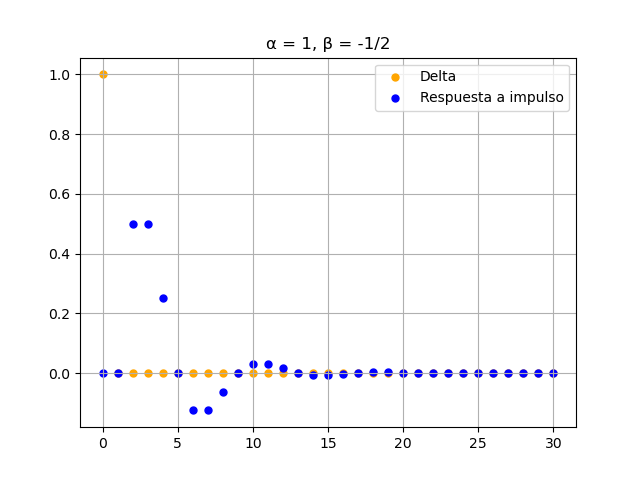
\includegraphics[width=\textwidth]{images/ej9_fig1_delta.png}
    \caption{Respuesta del sistema a señal impulso.}
    \end{minipage}
    \hfill
    \begin{minipage}[b]{0.49\textwidth}
    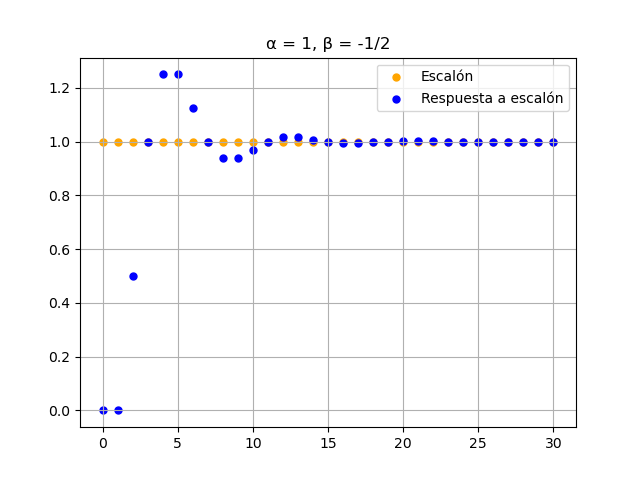
\includegraphics[width=\textwidth]{images/ej9_fig1_step.png}
    \caption{Respuesta del sistema a señal escalón.}
    \end{minipage}
\end{figure}

\begin{figure}[H]
    \centering
    \begin{minipage}[b]{0.49\textwidth}
    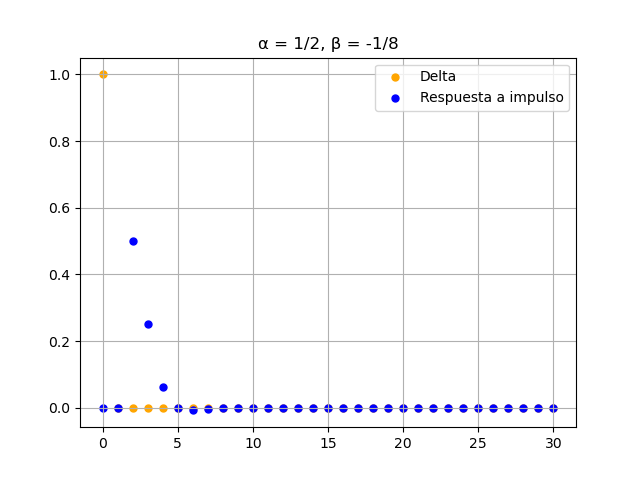
\includegraphics[width=\textwidth]{images/ej9_fig2_delta.png}
    \caption{Respuesta del sistema a señal impulso.}
    \end{minipage}
    \hfill
    \begin{minipage}[b]{0.49\textwidth}
    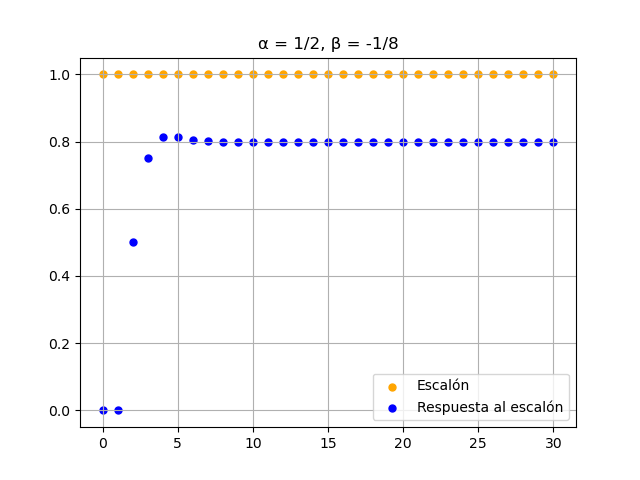
\includegraphics[width=\textwidth]{images/ej9_fig2_step.png}
    \caption{Respuesta del sistema a señal escalón.}
    \end{minipage}
\end{figure}

\begin{figure}[H]
    \centering
    \begin{minipage}[b]{0.49\textwidth}
    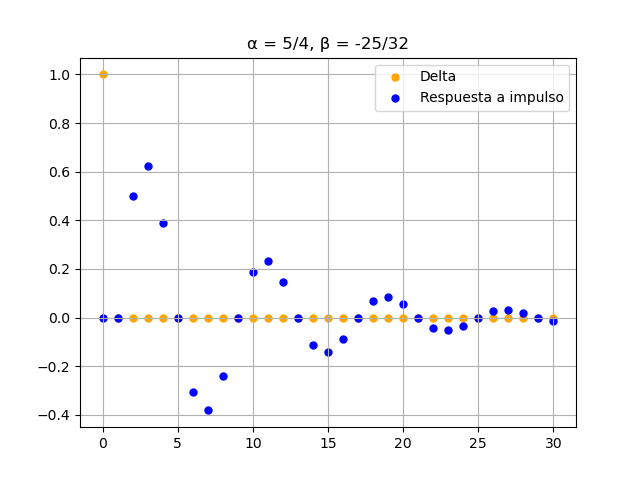
\includegraphics[width=\textwidth]{images/ej9_fig3_delta.png}
    \caption{Respuesta del sistema a señal impulso.}
    \end{minipage}
    \hfill
    \begin{minipage}[b]{0.49\textwidth}
    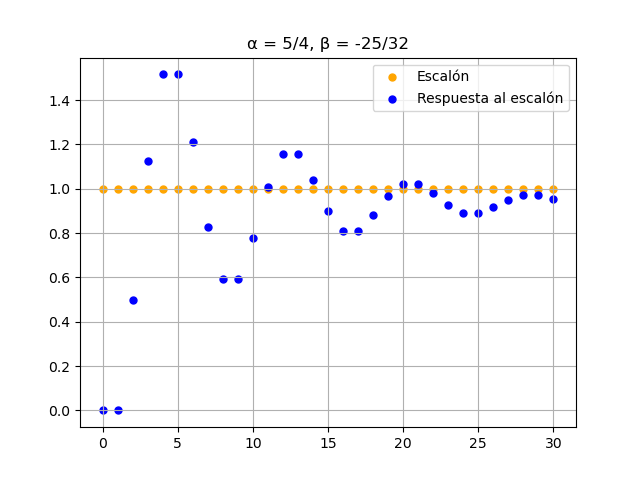
\includegraphics[width=\textwidth]{images/ej9_fig3_step.png}
    \caption{Respuesta del sistema a señal escalón.}
    \end{minipage}
\end{figure}

Observando las respuestas al impulso superpuestas:

\begin{figure}[H]
    \centering 
    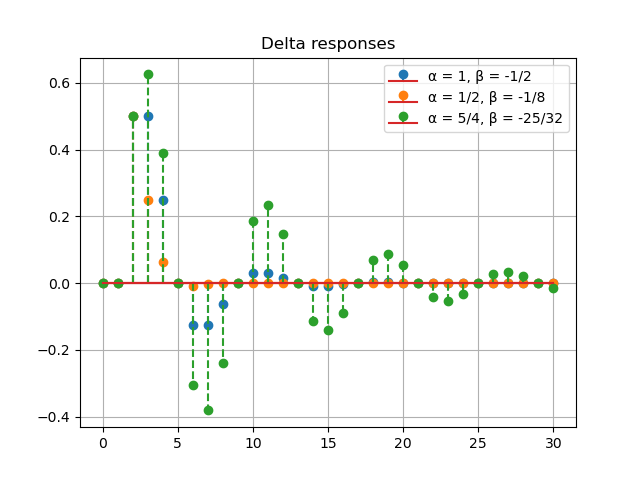
\includegraphics [scale=0.6]{images/ej9_all_delta.png} 
    \caption{Respuestas del sistema a la señal impulso}
\end{figure}

Se observa que todos los casos se corresponden, aproximadamente, con un periodo $T \sim 8$. De modo que:

$$f_{osc} \approx \frac{1}{8}$$

Se puede estimar la respuesta en frecuencia del sistema para todos los casos, y en particular al correspondiente a $\alpha  = 1, \beta = -\frac{1}{2}$, planteando
una señal de entrada $x(nT) = e^{jnwT}$, con T = 1, y realizando nuevamente un cálculo para la salida del sistema iterando en n. Como se trata de un sistema lineal, causal, dinámico y tiempo invariante 
(propiedades que se pueden determinar observando la expresión de la ecuación en diferencias), se debería llegar a que $y(n) =  H(w)e^{jwn}$. Iterando en un intervalo representativo de n podría estimarse la respuesta en frecuencia $H(w)$.

